% !TeX encoding = UTF-8
% !TeX program = pdflatex
% !BIB program = bibtex



\documentclass[english]{lni}

%\usepackage[english]{babel}
%\usepackage{dsthesis}

\usepackage{verbatim}

\usepackage{algorithm}
\usepackage[noend]{algpseudocode}
\usepackage{algorithmicx}


\usepackage{framed}
\usepackage{todonotes}
\usepackage{graphicx}
\usepackage{multirow}
\usepackage{tocloft}
\usepackage{longtable}
\usepackage{booktabs}
\usepackage{microtype}

%\usepackage{amssymb,amsmath,amsthm,amsfonts}
\usepackage{amsmath,amsfonts}
\newtheorem{definition}{Definition}
\newenvironment{proof}{\paragraph{Proof:}}{\hfill$\square$}
\newtheorem{theorem}{Theorem}

% DRAFT TOOLS
%\geometry{showframe}
\usepackage{todonotes}


\begin{document}
%%% Mehrere Autoren werden durch \and voneinander getrennt.
%%% Die Fußnote enthält die Adresse sowie eine E-Mail-Adresse.
%%% Das optionale Argument (sofern angegeben) wird für die Kopfzeile verwendet.
\title[Ein Kurztitel]{Extending K-Means Clustering with Ptolemy’s Inequality}
%% \subtitle{Untertitel / Subtitle} % if needed
 \author[1,2]{Max Pernklau}{firstname1.lastname1@affiliation1.org}{0000-0000-0000-0000}
 \author[2]{Nikita Averitchev}{firstname2.lastname2@affiliation2.org}{0000-0000-0000-0000}
 \author[3]{Christian Beecks}{firstname3.lastname3@affiliation1.org}{0000-0000-0000-0000}
% \author[1]{Firstname4 Lastname4}{firstname4.lastname4@affiliation1.org}{0000-0000-0000-0000}%
 \affil[1]{Universität 1\\Abteilung\\Straße\\Postleitzahl Ort\\Land}
 \affil[2]{University 2 \\Department\\Address\\Country}
 \affil[3]{University 3\\Department\\Address\\Country}
\maketitle

\begin{abstract}
Clustering is a fundamental data-analytical operation in the field of unsupervised learning. Given a database of unknown structure, clustering aims to discover the inherent structure of the data objects according to similarity, such that similar data objects are grouped together and dissimilar ones are separated in different groups or clusters. %The resulting groups, which are denoted as clusters, then represent the clustering structure of the database. A
Among the various approaches of clustering methods, we focus on partitioning methods, i.e. on the specific problem of \emph{k-means clustering}, which minimizes the intra-cluster variance. 
%where the Lloyd algorithm is a prominent and de facto standard implementation.
As the standard algorithmic approach to k-means clustering, namely the Lloyd algorithm, lacks on efficiency and scalability, various adaptations and modifications have been developed yielding to the family of fast k-means clustering algorithms. In this short paper, we extend the clustering algorithm proposed by Elkan with Ptolemy's inequality, which generalizes the triangle inequality, to prune unnecessary distance calculations. The aim of our short paper is not to compete with the state-of-the-art algorithmic solutions for the k-means clustering problem, but to investigate the potential of Ptolemy’s inequality to further enhancements in the standard algorithm’s performance, specifically in terms of reducing computations associated with distance evaluations.

\end{abstract}
\begin{keywords}
k-means clustering \and Lloyd algorithm \and Ptolemy's inequality %Keyword1 \and Keyword2
\end{keywords}
%%% Beginn des Artikeltexts

\todo{Americanize spelling (thesis uses chiefly British terms)}

\section{Introduction}

%intro
Clustering is a fundamental data-analytical operation in the domain of data science, where the basic task is to divide a set of data objects into different groups or clusters, such that objects within the same cluster have sufficient similarities, while objects in different clusters have significant differences. The collection of clusters reflects the inherent structure of the database and is denoted as clustering.

Clustering can be found in various scientific or economic application domains \cite{ezugwu2022comprehensive,oyewole2023data, gan2020data}, ranging from archaeology \cite{troiano2024comparative} and finance \cite{cai2016clustering} to industry \cite{lee2021technological} and zoology \cite{shen2021multivariate}, to name just a few. Especially in the field of unsupervised learning, clustering is utilized to extract structures from unlabeled data \cite{chander2023data}.

Alongside the diverse applications of clustering, unique domain-specific requirements and challenges arise, each of which can be addressed by leveraging different families of clustering approaches \cite{xu2015comprehensive,han2012data}. These approaches, ranging from partitioning and hierarchical methods to density-based, grid-based and graph-based methods, are designed to accommodate varying data characteristics and application-related requirements to facilitate efficient cluster analyses across diverse domains.

%different algorithms/problems
%kmeans/lloyd
%fast algorithms
%inefficient: distance calculations
%our proposal: ptolemaic
%our purpose

In this short paper, we focus on partitioning methods due to their simplicity in terms of interpretability and implementability \cite{DBLP:conf/iiwas/BeecksBHLSD22}. In this field, the \emph{k-means algorithm} \cite{bock2007clustering,hans2008origins,DBLP:journals/prl/Jain10,steinley2006k} has become one of the most influential clustering techniques \cite{DBLP:journals/kais/WuKQGYMMNLYZSHS08,olukanmi2019rethinking}. Although the term "k-means algorithm" is explicitly credited to MacQueen \cite{macqueen1967}, its origins trace back to Steinhaus \cite{steinhaus1956division} in 1956, with its first application to data clustering by Forgy \cite{forgy1965cluster} in 1965. The widely recognized version in use today is the \emph{Lloyd algorithm} \cite{DBLP:journals/tit/Lloyd82}, introduced in 1982.

With the proliferation of complex data sources and the growing demand for more efficient clustering techniques, numerous \emph{fast k-means algorithms} have been introduced \cite{DBLP:conf/icml/Elkan03,DBLP:conf/sdm/Hamerly10,drake2012accelerated,hamerly2015accelerating,DBLP:conf/icml/NewlingF16,DBLP:conf/icml/DingZSMM15}. These methods are designed to achieve exact clustering results with significantly reduced computational cost. Moreover, they do not require any form of precomputation, making them directly applicable across a wide range of scenarios.

%contribution

%structure


\newpage

\section{Related Work}


\section{Foundations of Ptolemaic Indexing}


\todo{explain Hetland's lower (upper) bound notation ($d^-$ and $d^+$)}
\begin{theorem}[Ptolemaic Bounds]
	\label{thm4.2}
	\todo{we might want to explain what the points are supposed to do before showing this theorem.
		Or, alternatively, we just present this as a purely mathematical statement with no preceding motivation.}
	Let \(a, b, c, c' \in \mathbb{R}^n\) and let \(d(\cdot, \cdot)\) be the Euclidean distance. The distance \(d(a, c')\) can be bounded as follows:
	\begin{gather}
		\frac{1}{d(b, c)} \cdot \max \left\{
		\begin{array}{l}
			d(a, b)^- \cdot d(c, c') - d(a, c)^+ \cdot d(b, c'), \\
			d(a, c)^- \cdot d(b, c') - d(a, b)^+ \cdot d(c, c')
		\end{array}
		\right\} \leq d(a, c')
	\end{gather}
	and
	\begin{gather}
		d(a, c') \leq \frac{1}{d(b, c)} \cdot \left( d(a, c) \cdot d(b, c') + d(a, b) \cdot d(c, c') \right)
	\end{gather}
\end{theorem}
\begin{proof}
	\todo{convert to passive voice}
	\todo{expand context to summarize all steps that lead to this proof}
	The lower bound corresponds to the derivation in equation \ref{eq4.4} and corresponds to the arrangement of the two pivot objects. Replace some distances with the respective lower or upper bound for the distance. The lower bounds can be used as they are always smaller than the exact distance. The upper bound must be used due to the subtraction. This means that the inequality still applies. The upper bound is obtained by using Ptolemy's inequality:

	\begin{equation*}
		\begin{aligned}
			\label{eq4.7}
			d(a,c') \cdot d(b,c) & \leq d(a, c) \cdot d(b, c') + d(a, b) \cdot d(c, c')                \\
			d(a,c')              & \leq \frac{d(a, c) \cdot d(b, c') + d(a, b) \cdot d(c, c')}{d(b,c)}
		\end{aligned}
	\end{equation*}
	By replacing some distances with upper boundaries you get the desired upper boundaries.
\end{proof}




\section{Applying Ptolemy's Inequality to the Elkan's Algorithm}




\subsection{Integration in k-Means}
Theorem \ref{thm4.2} will now be applied in a similar context to Elkan's algorithm \ref{alg:elkan}, with the goal of integrating these new bounds into steps 5 and 6 of the algorithm.

Consider the data set \(D = \{x_1, \ldots, x_n\}\). For each \(x_i\), there is an upper \(u_i\) and lower bounds \(l_{ij}\) as in Elkan's algorithm. The new cluster center assigned in a iteration is denoted by \(c_i^{\text{new}}\), and the old cluster center by \(c_i^{\text{old}}\). To use Ptolemy's Inequality, one additional point is needed. The idea is to use an even older cluster center \(c_i^{\text{old,old}}\) obtained two iterations ago.

Overall, to obtain a new upper bound for the distance between the datapoint \(x_i\) and the new cluster center \(c_j^{\text{new}}\), consider the old cluster center \(c_j^{\text{old}}\) from the last iteration to which \(x_i\) was assigned, and the even older cluster center \(c_j^{\text{old,old}}\) from two iterations ago. Utilize the old upper bounds that were valid for the respective iteration.

\begin{equation*}
	\begin{aligned}
		d(x_i,c_i^{old})      & \leq u_i^{old}      \\
		d(x_i,c_i^{old, old}) & \leq u_i^{old, old}
	\end{aligned}
\end{equation*}

Similarly, to obtain a new lower bound for the distance between the datapoint \(x_i\) and the new cluster center \(c_j^{\text{new}}\), the old lower bounds from the respective iterations are used:

\begin{equation*}
	\begin{aligned}
		l_{i,j}^{\text{old}}     & \leq d(x_i, c_j^{\text{old}})     \\
		l_{i,j}^{\text{old,old}} & \leq d(x_i, c_j^{\text{old,old}})
	\end{aligned}
\end{equation*}

Using Theorem \ref{thm4.2}, the following upper bound for the distance are obtained:
\begin{equation}
	\label{eq4.7}
	d(x_i, c_j^{\text{new}}) \leq u_i^{\text{new}} = \frac{1}{d(c_j^{\text{old}}, c_j^{\text{old,old}})} \cdot \left( u_i^{\text{old}} \cdot d(c_j^{\text{new}}, c_j^{\text{old,old}}) + u_i^{\text{old,old}} \cdot d(c_j^{\text{new}}, c_j^{\text{old}}) \right)
\end{equation}

and the new lower bound:
\begin{equation}
	\label{eq4.8}
	d(x_i, c_j^{\text{new}}) \geq l_{i,j}^{\text{new}} = \frac{1}{d(c_j^{\text{old}}, c_j^{\text{old,old}})} \cdot \max \left\{
	\begin{array}{l}
		l_{i,j}^{\text{old,old}} \cdot d(c_j^{\text{old}}, c_j^{\text{new}}) - u_i^{\text{old}} \cdot d(c_j^{\text{new}}, c_j^{\text{old,old}}), \\
		l_{i,j}^{\text{old}} \cdot d(c_j^{\text{new}}, c_j^{\text{old,old}}) - u_i^{\text{old,old}} \cdot d(c_j^{\text{old}}, c_j^{\text{new}})
	\end{array}
	\right\}
\end{equation}

You can see that the old upper boundaries are required to calculate the new lower boundaries.

Let us now look at how these bounds can be integrated into Elkan's algorithm. It is important to save not only the cluster centres and the bounds of the last iteration, but also those of the penultimate iteration.

At the beginning, all distances to all cluster centres are calculated in the first iteration. The upper bound is set by the distance to the nearest cluster centre, and the lower bounds are determined by the direct distances from the point to the respective cluster centres. An iteration is then performed as with Elkan, which means that bounds from two iterations are now available. This makes it possible to apply the new bounds from equations \ref{eq4.7} and \ref{eq4.8}. The algorithm then iterates, as in the original Elkan algorithm using updating with new update conditions, until the cluster centres converge or a specified number of iterations is reached. It is always important to check whether $d(c_j^{\text{old}}, c_j^{\text{old,old}}) \neq 0$. If this is the case, the update is carried out as for Elkan. The algorithm is displayed in Algorithm \ref{alg:ptolemy}.




\begin{algorithm}
	\caption{Elkan's Algorithm extended with Ptolemy's inequality}
	\label{alg:ptolemy}

	\begin{algorithmic}

		\State \textbf{Initialization:} Initialize all cluster centers. For each point $x_i$ and each center $c_j$, set the lower bound $l(x_i,c_j)$ and the upper bound $u(x_i)$. Assign each $x_i$ to the nearest cluster $C_j$ such that $c(x_i) = \arg \min_j d(x_i, c_j)$, utilizing Lemma 1 to minimize distance calculations. Set $r(x_i) = \text{true}$ for all points.

		\State \textbf{Step 0:} Compute one iteration of Elkan's algorithm. Save old upper and lower bounds of the last two iterations.
		\Repeat
		\State \textbf{Step 1:}  Compute distances $d(c_i, c_j)$ between all centers, and calculate $s(c_i) = \frac{1}{2} \min_{c_j \neq c_i} d(c_i, c_j)$ for each center $c_i$.
		\Statex
		\State \textbf{Step 2:}  Retain points $x_i$ in their current clusters if $u(x_i) \leq s(c(x_i))$.
		\Statex
		\State \textbf{Step 3:}  For remaining points, consider $x_i$ for reassignment if:
		\begin{itemize}
			\item $c_j \neq c(x_i)$,
			\item $u(x_i) > l(x_i, c_j)$, and
			\item $u(x_i) > \frac{1}{2}d(c(x_i), c_j)$.
		\end{itemize}
		\Statex
		\State \textbf{Step 3a:}  If $r(x_i)$ is true, compute $d(x_i, c(x_i))$. Set $r(x_i) = \text{false}$. Otherwise, $u(x_i) =d(x_i, c(x_i))$
		\Statex
		\State \textbf{Step 3b:} If $d(x_i, c(x_i)) > l(x_i, c_j)$ or $d(x_i, c(x_i)) > \frac{1}{2}d(c(x_i), c_j)$, compute $d(x_i, c_j)$. Reassign $x_i$ to $C_j$ if $d(x_i, c_j) < d(x_i, c(x_i))$.
		\Statex
		\State \textbf{Step 4:} Compute the cluster centers as the centroids of the corresponding clusters $c'_j$.
		\Statex
		\State \textbf{Step 5:} If distance between two older cluster is not 0. Update lower bounds by using equation \ref{eq4.8}. Otherwise, update like in Elkan. Save the old lower bounds of the two last iterations.
		\Statex
		\State \textbf{Step 6:} If distance between two older cluster is not 0. Update upper bounds by using equation \ref{eq4.7}. Otherwise, update like in Elkan. Reset $r(x_i) = \text{true}$. Save old cluster and upper bounds of the last two iterations.
		\Statex
		\State \textbf{Step 7:} Replace each center $c_j$ with $c'_j$.

		\Until{convergence}

	\end{algorithmic}
\end{algorithm}





\section{Preliminary Results}

\begin{figure}
  \centering
  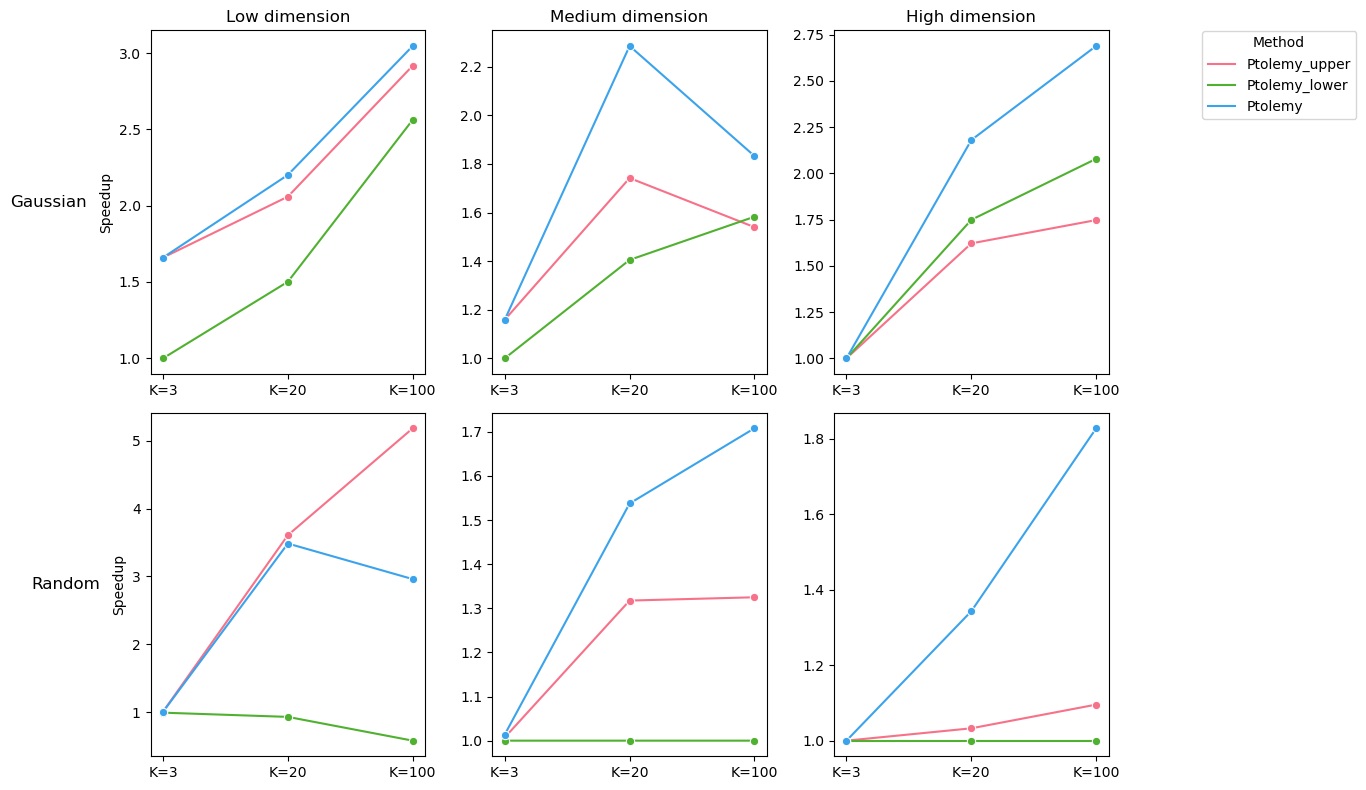
\includegraphics[width=.8\textwidth]{fig/gaussia+random.png}
  \caption{}
  \label{fig:gauss_univariate}
\end{figure}

\begin{figure}
  \centering
  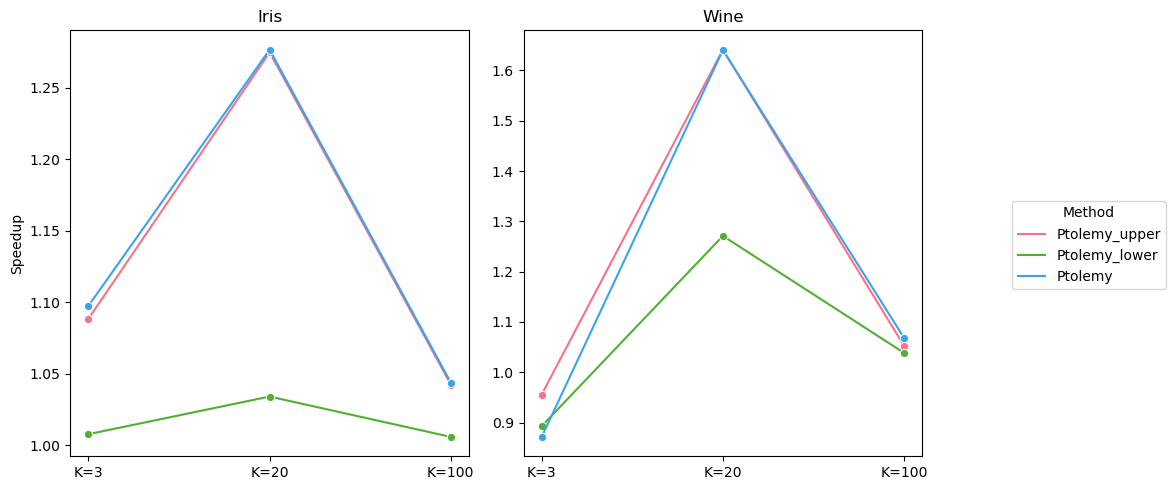
\includegraphics[width=.8\textwidth]{fig/wine+iris.png}
  \caption{}
  \label{fig:data}
\end{figure}

\todo{
    Experiments to show:
    - iris, wine, gaussian, uniform
    (moons, circles aren't a good fit for k-means -- is that reason enough to exclude them?)
}

\todo{we should mention that the Pto\_low version performs worse in every test (but one), but we do not need to include it in the comparison between Elkan and Our Work}

\todo{compile a graph that summarizes the four pages of tables}

\todo{How much do we "trust" these results, provided that each test configuration ( [k choice]x[dataset]x[algorithm]) was only run once?
We might need to repeat and average over these experiments.
TBD
}



\section{Conclusions and Future Work}


%%% Angabe der .bib-Datei (ohne Endung) / State .bib file (im Falle der Nutzung von BibTeX)
\bibliography{references,bibliography_thesis,bibliography_iiwas}
%% \printbibliography % im Falle der Nutzung von biblatex
\end{document}
